\documentclass[a4paper,14pt,oneside,final]{extarticle}
\usepackage[top=2cm, bottom=2cm, left=3cm, right=1cm]{geometry}
\usepackage{scrextend}

\usepackage[T2A,T1]{fontenc}
\usepackage[ukrainian,russian,english]{babel}
\usepackage{tempora}
\usepackage{fontspec}
\setmainfont{tempora}

% Зачем: Отключает использование изменяемых межсловных пробелов.
% Почему: Так не принято делать в текстах на русском языке.
\frenchspacing

\usepackage{indentfirst}
\setlength{\parindent}{1.25cm}
\renewcommand{\baselinestretch}{1.5}

% Header
\usepackage{fancyhdr}
\pagestyle{fancy}
\fancyhead{}
\fancyfoot{}
\fancyhead[R]{\small \selectfont \thepage}
\renewcommand{\headrulewidth}{0pt}

% Captions
\usepackage{chngcntr}
\counterwithin{figure}{section}
\counterwithin{table}{section}
\usepackage[tableposition=top]{caption}
\usepackage{subcaption}
\DeclareCaptionLabelFormat{gostfigure}{Рисунок #2}
\DeclareCaptionLabelFormat{gosttable}{Таблиця #2}
\DeclareCaptionLabelSeparator{gost}{~---~}
\captionsetup{labelsep=gost}
\captionsetup[figure]{labelformat=gostfigure}
\captionsetup[table]{labelformat=gosttable}
\renewcommand{\thesubfigure}{\asbuk{subfigure}}

% Sections
\usepackage[explicit]{titlesec}
\newcommand{\sectionbreak}{\clearpage}

\titleformat{\section}
  {\centering}{\thesection \quad}{0pt}{\MakeUppercase{#1}}
\titleformat{\subsection}[block]
  {\bfseries}{\thesubsection \quad #1}{0cm}{}

\titlespacing{\section} {0cm}{0cm}{21pt}
\titlespacing{\subsection} {\parindent}{21pt}{0cm}
\titlespacing{\subsubsection} {\parindent}{0cm}{0cm}

% Lists
\usepackage{enumitem}
\renewcommand\labelitemi{--}
\setlist[itemize]{noitemsep, topsep=0pt, wide}
\setlist[enumerate]{noitemsep, topsep=0pt, wide, label=\arabic*}
\setlist[description]{labelsep=0pt, noitemsep, topsep=0pt, leftmargin=2\parindent, labelindent=\parindent, labelwidth=\parindent, font=\normalfont}

% Toc
\usepackage{tocloft}
\tocloftpagestyle{fancy}
\renewcommand{\cfttoctitlefont}{}
\setlength{\cftbeforesecskip}{0pt}
\renewcommand{\cftsecfont}{}
\renewcommand{\cftsecpagefont}{}
\renewcommand{\cftsecleader}{\cftdotfill{\cftdotsep}}

\usepackage{float}
\usepackage{pgfplots}
\usepackage{graphicx}
\usepackage{multirow}
\usepackage{amssymb,amsfonts,amsmath,amsthm}
\usepackage{csquotes}

\usepackage{listings}
\lstset{basicstyle=\footnotesize\ttfamily,breaklines=true}
\lstset{language=Matlab}

\usepackage[
	backend=biber,
	sorting=none,
	language=auto,
	autolang=other
]{biblatex}
\DeclareFieldFormat{labelnumberwidth}{#1}

\lstdefinelanguage{Python}{
  keywords={and, break, class, continue, def, yield, del, elif, else, except, exec, finally, for, from, global, if, import, in, lambda, not, or, pass, print, raise, return, try, while, assert, with},
  keywordstyle=\color{NavyBlue}\bfseries,
  ndkeywords={True, False},
  ndkeywordstyle=\color{BurntOrange}\bfseries,
  emph={as},
  emphstyle={\color{OrangeRed}},
  identifierstyle=\color{black},
  sensitive=true,
  commentstyle=\color{gray}\ttfamily,
  comment=[l]{\#},
  morecomment=[s]{/*}{*/},
  stringstyle=\color{ForestGreen}\ttfamily,
  morestring=[b]',
  morestring=[s]{"""*}{*"""},
}


\newcommand{\labnumber}{1} % first lab
\documentclass[a4paper,14pt,oneside,final]{extarticle}
\usepackage[top=2cm, bottom=2cm, left=3cm, right=1cm]{geometry}
\usepackage{scrextend}

\usepackage[T2A,T1]{fontenc}
\usepackage[ukrainian,russian,english]{babel}
\usepackage{tempora}
\usepackage{fontspec}
\setmainfont{tempora}

% Зачем: Отключает использование изменяемых межсловных пробелов.
% Почему: Так не принято делать в текстах на русском языке.
\frenchspacing

\usepackage{indentfirst}
\setlength{\parindent}{1.25cm}
\renewcommand{\baselinestretch}{1.5}

% Header
\usepackage{fancyhdr}
\pagestyle{fancy}
\fancyhead{}
\fancyfoot{}
\fancyhead[R]{\small \selectfont \thepage}
\renewcommand{\headrulewidth}{0pt}

% Captions
\usepackage{chngcntr}
\counterwithin{figure}{section}
\counterwithin{table}{section}
\usepackage[tableposition=top]{caption}
\usepackage{subcaption}
\DeclareCaptionLabelFormat{gostfigure}{Рисунок #2}
\DeclareCaptionLabelFormat{gosttable}{Таблиця #2}
\DeclareCaptionLabelSeparator{gost}{~---~}
\captionsetup{labelsep=gost}
\captionsetup[figure]{labelformat=gostfigure}
\captionsetup[table]{labelformat=gosttable}
\renewcommand{\thesubfigure}{\asbuk{subfigure}}

% Sections
\usepackage[explicit]{titlesec}
\newcommand{\sectionbreak}{\clearpage}

\titleformat{\section}
  {\centering}{\thesection \quad}{0pt}{\MakeUppercase{#1}}
\titleformat{\subsection}[block]
  {\bfseries}{\thesubsection \quad #1}{0cm}{}

\titlespacing{\section} {0cm}{0cm}{21pt}
\titlespacing{\subsection} {\parindent}{21pt}{0cm}
\titlespacing{\subsubsection} {\parindent}{0cm}{0cm}

% Lists
\usepackage{enumitem}
\renewcommand\labelitemi{--}
\setlist[itemize]{noitemsep, topsep=0pt, wide}
\setlist[enumerate]{noitemsep, topsep=0pt, wide, label=\arabic*}
\setlist[description]{labelsep=0pt, noitemsep, topsep=0pt, leftmargin=2\parindent, labelindent=\parindent, labelwidth=\parindent, font=\normalfont}

% Toc
\usepackage{tocloft}
\tocloftpagestyle{fancy}
\renewcommand{\cfttoctitlefont}{}
\setlength{\cftbeforesecskip}{0pt}
\renewcommand{\cftsecfont}{}
\renewcommand{\cftsecpagefont}{}
\renewcommand{\cftsecleader}{\cftdotfill{\cftdotsep}}

\newcommand{\khpistudentgroup}{КН-34г}
\newcommand{\khpistudentname}{Чепурний~А.~С.}

\newcommand{\khpidepartment}{Програмна інженерія та інформаційні технології управління}
\newcommand{\khpititlewhat}{
	Лабораторна робота №\labnumber \\
	з предмету <<Моделювання систем>>
}
\newcommand{\khpititlewho}{
	Виконав: \\
	\hspace*{\parindent} ст. групи \khpistudentgroup \\
	\hspace*{\parindent} \khpistudentname \\
	Перевірила: \\
	\hspace*{\parindent} ст. в. каф. ПІІТУ \\
	\hspace*{\parindent} Єршова~С.~І. \\
	\hspace*{\parindent} ас. каф. ПІІТУ \\
	\hspace*{\parindent} Литвинова~Ю.~С. \\
}



\graphicspath{{figures/}}

\begin{document}
\Ukrainian

\begin{titlepage}

\begin{center}
	МІНІСТЕРСТВО ОСВІТИ І НАУКИ УКРАЇНИ \\
	НАЦІОНАЛЬНИЙ ТЕХНІЧНИЙ УНІВЕРСИТЕТ \\
	«ХАРКІВСЬКИЙ ПОЛІТЕХНІЧНИЙ ІНСТИТУТ» \\[0.5cm]
	Кафедра <<\khpidepartment>> \\
\end{center}

\vspace{6cm}

\begin{center}
	\khpititlewhat
\end{center}

\vspace{3cm}

\begin{addmargin}[10cm]{0cm}
	\khpititlewho
\end{addmargin}

\vspace{\fill}

\begin{center}
	Харків \the\year
\end{center}

\end{titlepage}

\addtocounter{page}{1}

\section*{Моделювання предметної області}
\subsubsection*{Мета}
Знайомство зі стандартом IDEF5 та його використання.
\subsubsection*{Постановка задач}
\begin{enumerate}
  \item Провести аналіз предметної області згідно індивідуальному завданню виділити окремі сутності та перелік значень. 
  Перелік предметних областей наведено нижче. 
  Номер області відповідає номеру у журналі академічної групи.
  \item Розробити модель бази даних для обраної предметної області.
  \item Розробити онтологію для обраної предметної області згідно стандарту IDEF5, обґрунтувати вибір типу схеми.
\end{enumerate}

\begin{center}
Варіант 16 --- Управління страховими договорами.
\end{center}

\subsection*{Аналіз предметної області}
Предметною областю є управління медичними страховими договорами приєднання.

Глосарій предметної області:
\begin{enumerate}
  \item Страховик --- страхова компанія, яка надає послуги страхування. 
  \item Страхувальник --- фізична особа, яка уклала договір про страхування здоров'я та працездатності на свою користь.
  \item Страхова сума --- грошова сума, в межах якої страховик відповідно до умов договору страхування зобов'язаний здійснювати страхові виплати при настанні страхового випадку. 
  \item Страховий випадок --- подія, передбачена договором страхування, яка відбулася після набуття чинності договору страхування і з настанням якої виникає обов'язок страховика здійснити страхову виплату страхувальнику.
  \item Страховий ризик --- певна подія, на випадок якої проводиться страхування і яка має ознаки ймовірності та випадковості настання.
  \item Медичне страхування --- тип страхування від ризику витрат, пов'язаних із отриманням медичної допомоги.
  \item Договір приєднання --- договір, умови якого встановлені однією із сторін у формулярах або інших стандартних формах, який може бути укладений лише шляхом приєднання другої сторони до запропонованого договору в цілому. 
  \item Договір страхування --- договір приєднання медичного страхування. 
\end{enumerate}

При виникненні страхового випадку страховик гарантує оплату медичної допомоги, за рахунок накопичених страхувальниками коштів. 
Медичне страхування дозволяє гарантувати громадянину безкоштовне надання певного обсягу медичних послуг, при виникненні страхового випадку (порушення здоров'я), за наявності договору зі страховиком. 
Остання несе витрати з оплати випадку надання медичної допомоги, з моменту сплати громадянином першого внеску до відповідного фонду.

\subsection*{Розробка моделі даних для обраної предметної області}
Згідно заданій предметній області була розроблена концептуальна модель бази даних, що зображена на рисунку~\ref{fig:er}.

\begin{figure}[H]
    \centering
        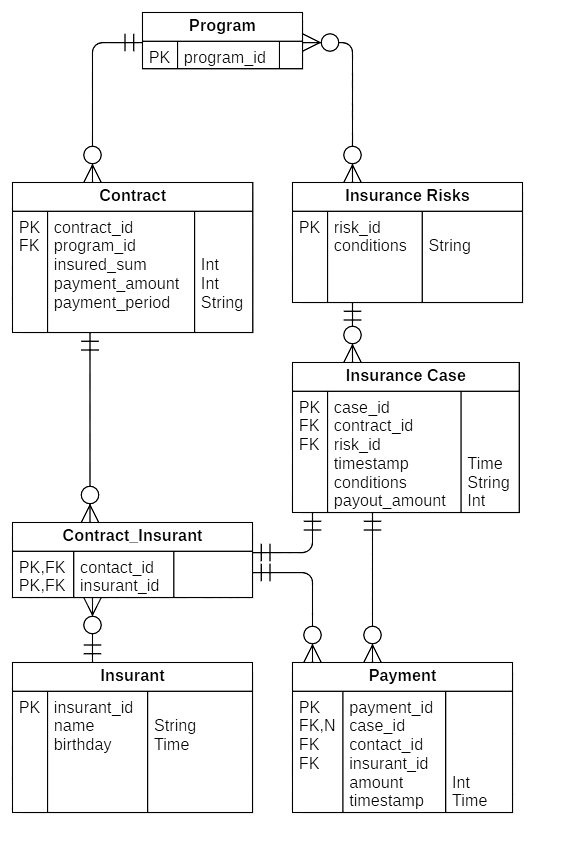
\includegraphics[width=0.6\linewidth]{er}
    \caption{Концептуальна модель бази даних}
    \label{fig:er}
\end{figure}

Перелік сутностей в моделі даних: 
\begin{itemize}
  \item \texttt{Program} --- страхова програма;
  \item \texttt{Contract} --- страховий договір приєднання;
  \item \texttt{Insurance Risks} --- страхові ризики;
  \item \texttt{Insurance Case} --- страховий випадок;
  \item \texttt{Insurant} --- страхувальник;
  \item \texttt{Payment} --- виплати.
\end{itemize}

\subsection*{Розробка онтології для обраної предметної області}
Для обраної предметної області була розроблена онтологія згідно стандарту IDEF5. 
Діаграми стану, взаємозв'язку, композиціі та класифікації договору страхування представлені на рисунках~\ref{fig:idef_state}, \ref{fig:idef_relation}, \ref{fig:idef_composition}, \ref{fig:idef_classification}.

\begin{figure}[H]
    \centering
        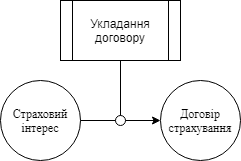
\includegraphics{idef_state}
    \caption{Діаграма стану укладання договору}
    \label{fig:idef_state}
\end{figure}

\begin{figure}[H]
    \centering
        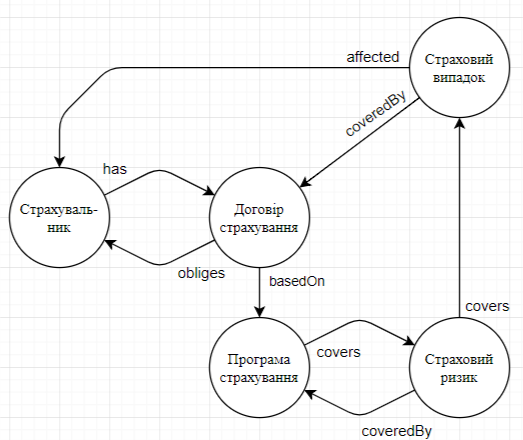
\includegraphics[width=0.7\linewidth]{idef_relation}
    \caption{Взаємозв'язок договору страхування}
    \label{fig:idef_relation}
\end{figure}

\begin{figure}[H]
    \centering
        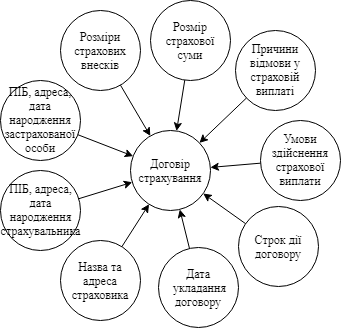
\includegraphics[width=0.6\linewidth]{idef_composition}
    \caption{Композиційна схема договору страхування}
    \label{fig:idef_composition}
\end{figure}

\begin{figure}[H]
    \centering
        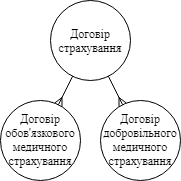
\includegraphics{idef_classification}
    \caption{Класифікація договорів страхування}
    \label{fig:idef_classification}
\end{figure}

\subsection*{Висновки}
У ході виконання лабораторної роботи було виконано аналіз предметної області, що пов'язана із управлінням страховими договорами. Була розроблена онтологія предметної області у вигляді діаграми взаємозв'язку, що відображає зв'язки між сутностями предметної області та діаграми станів. Також була розроблена фізична модель даних системи управління страховими договорами.

\end{document}
